\apendice{Especificación de Requisitos}

\section{Introducción}

En este anexo se describen los servicios que ha de ofrecer la aplicación \emph{SurveyingPointCode} y las restricciones asociadas a su funcionamiento. La función principal de la especificación de requisitos es servir como medio de comunicación entre clientes, usuarios, y desarrolladores.

Se recogerán todos los requisitos funcionales y no funcionales.

\section{Objetivos generales}
En este apartado se detallarán los distintos objetivos generales que se persiguen con este proyecto:

\begin{itemize}
\item Definir una codificación de puntos en un levantamiento topográfico que permita la automatización del proceso e delineación y mejore la toma de datos en campo.
\item Desarrollar una aplicación Web, que permita la conversión de un archivo de campo, con datos topográficos a un archivo DXF, interpretando la codificación y generando todos los elementos del dibujo de forma automática.
\item Trabajar con archivos personalizados del usuario como: configuración de la conversión y archivo DXF de símbolos, para la obtención del DXF final.
\item El usuario debe estar registrado, para acceder a la aplicación.
\end{itemize}

\section{Catalogo de requisitos}

A continuación,  definirán tanto los requisitos funcionales como los no
funcionales necesarios para cumplir con los objetivos generales.

\subsection{Requisitos funcionales}

\begin{itemize}
\item \textbf{RF-1 Registro de usuario: }el usuario debe poder 		registrarse, mediante un nombre, un e-mail y una contraseña.

\item \textbf{RF-2 \emph{Login} de usuario: }el usuario debe poder 	\emph{logearse}, mediante un e-mail y una contraseña.



\item \textbf{RF-3 Carga de archivos: }el usuario debe ser capaz de gestionar diferentes tipos de archivos: de campo, de configuración de la conversión y de símbolos.

\begin{itemize}
\item \textbf{RF-3.1 Carga de archivo de campo: }el usuario debe poder cargar este archivo con los datos de un levantamiento topográfico, indicando su validez y en caso contrario, indicando cual es su error. Este archivo es obligatorio.

\item \textbf{RF-3.2 Carga de archivo de configuración: }el usuario debe poder cargar este archivo con los datos de una configuración personalizada para la conversión, indicando su validez y en caso contrario, indicando cual es su error. Este archivo es opcional.

\item \textbf{RF-3.3 Carga de archivo DXF con simbología: }el usuario debe poder cargar este archivo DXF con símbolos personalizados, indicando su validez y en caso contrario, indicando cual es su error. Este archivo es opcional.
	
\end{itemize}

\item \textbf{RF-4 Conversión: }el usuario debe ser capaz de generar un archivo DXF, partiendo del archivo de campo, pudiendo configurar esa conversión utilizando los archivos opcionales. Debe también existir la posibilidad de configurar desde cero o modificar una configuración de la conversión existente a través de la interfaz gráfica. El usuario debe poder elegir la versión de CAD para el DXF a generar, y ponerle un nombre personalizado al archivo generado.

\begin{itemize}

\item \textbf{RF-4.1 Asociar capas y colores: }el usuario debe poder asociar capas y colores, a los códigos, a través del archivo configuración de la conversión o de la interfaz. 

\item \textbf{RF-4.2 Asociar símbolos: }el usuario debe poder asociar símbolos a los códigos. Previamente debe haber cargado un archivo válido con símbolos. 

\item \textbf{RF-4.3 Elección de versión de CAD: }el usuario debe poder elegir la versión de CAD para generar el DXF, a través de un desplegable con las versiones disponibles.

\item \textbf{RF-4.4 Elección de nombre del archivo DXF generado: }el usuario debe poder dar un nombre personalizado al archivo DXF generado.

\end{itemize}

\item \textbf{RF-5 Descarga de archivos :} el usuario debe poder descargar los archivos generados a su equipo de forma individual o varios archivos en formato comprimido.


\item \textbf{RF-6 \emph{Logout} del usuario: }el usuario debe poder cerrar la sesión.

\item \textbf{RF-7 Limpieza de archivos almacenados en el servidor: }la aplicación debe eliminar los archivos utilizados durante la sesión, al cerrarse la sesión.

\end{itemize}



\subsection{Requisitos no funcionales}

\begin{itemize}
\item \textbf{RNF-1 Usabilidad: }la aplicación debe ser intuitiva, con una curva baja de aprendizaje y mensajes de errores claros para el usuario.

\item \textbf{RNF-2 Soporte: }la aplicación debe funcionar en los navegadores Web más usuales, como: Google Chrome, Mozilla Firefox y Microsoft Edge.

\item \textbf{RNF-3 Rendimiento: }la aplicación debe tener unos tiempos de conversión del archivo mínimos, por ejemplo, con archivos de campo de tamaño grande, 5.000 puntos, debe realizar la conversión en no más de 5 segundos.

\item \textbf{RNF-4 Escalabilidad: }la aplicación debe ser desarrollada de manera que permita la escalabilidad de la misma de forma sencilla.

\item \textbf{RNF-5 Seguridad:} la aplicación debe gestionar de forma adecuada todos los datos sensibles, como claves, tokens, etc.

\end{itemize}

\section{Especificación de requisitos}

A continuación se mostrarán los diagramas de casos de uso y el detalle de cada uno de ellos.


\subsection{Actores}

En este sistema, existe un actor que interactuará con el sistema, y el propio sistema.


\subsection{Casos de uso}
\imagen{CU-0}{Diagrama de general de casos de uso }

\imagen{CU-1}{Diagrama de caso de uso CU-01}
\strut
\begin{longtable}[H]{@{}ll@{}}
\toprule
\begin{minipage}[b]{0.23\columnwidth}\raggedright\strut
\textbf{CU-01}\strut
\end{minipage} & \begin{minipage}[b]{0.71\columnwidth}\raggedright\strut
\textbf{Registro del usuario}\strut
\end{minipage}\tabularnewline
\midrule
\endhead
\begin{minipage}[t]{0.23\columnwidth}\raggedright\strut
\textbf{Versión}\strut
\end{minipage} & \begin{minipage}[t]{0.71\columnwidth}\raggedright\strut
1.0\strut
\end{minipage}\tabularnewline
\begin{minipage}[t]{0.23\columnwidth}\raggedright\strut
\textbf{Autor}\strut
\end{minipage} & \begin{minipage}[t]{0.71\columnwidth}\raggedright\strut
José Eduardo Risco Sánchez-Cortés\strut
\end{minipage}\tabularnewline
\begin{minipage}[t]{0.23\columnwidth}\raggedright\strut
\textbf{Requisitos asociados}\strut
\end{minipage} & \begin{minipage}[t]{0.71\columnwidth}\raggedright\strut
RF-1\strut
\end{minipage}\tabularnewline
\begin{minipage}[t]{0.23\columnwidth}\raggedright\strut
\textbf{Descripción}\strut
\end{minipage} & \begin{minipage}[t]{0.71\columnwidth}\raggedright\strut
Permite al usuario registrarse.\strut
\end{minipage}\tabularnewline
\begin{minipage}[t]{0.23\columnwidth}\raggedright\strut
\textbf{Precondición}\strut
\end{minipage} & \begin{minipage}[t]{0.71\columnwidth}\raggedright\strut
El usuario no debe estar \emph{logeado}.\strut
\end{minipage}\tabularnewline
\begin{minipage}[t]{0.23\columnwidth}%\raggedright\strut
\textbf{Acciones}\strut
\end{minipage} & \begin{minipage}[t]{0.71\columnwidth}%\raggedright\strut
\begin{enumerate}
\def\labelenumi{\arabic{enumi}.}
\tightlist
\item
  El usuario entra en la aplicación y accede a la página de registro.
\item
  Introduce su nombre, e-mail, contraseña y confirma esta.
\item
  El usuario confirma el registro con el botón \emph{Register}
\end{enumerate}\strut
\end{minipage}\tabularnewline
\begin{minipage}[t]{0.23\columnwidth}%\raggedright\strut
\textbf{Postcondición}\strut
\end{minipage} & \begin{minipage}[t]{0.71\columnwidth}%\raggedright\strut
\begin{itemize}
\tightlist
\item
  La aplicación va a la pantalla de \emph{Login}
\item
  mensaje: \textit{You are now a registered user!}.
\end{itemize}\strut

\end{minipage}\tabularnewline
\begin{minipage}[t]{0.23\columnwidth}\raggedright\strut
\textbf{Excepciones}\strut
\end{minipage} & \begin{minipage}[t]{0.71\columnwidth}%\raggedright\strut
\begin{itemize}
\tightlist
\item
  mensaje: \textit{Please use a different username.}
\item
  mensaje: \textit{Please use a different email address.}
\item
  mensaje: \textit{Field must be equal to password.}  
  
\end{itemize}\strut
\end{minipage}\tabularnewline
\begin{minipage}[t]{0.23\columnwidth}\raggedright\strut
\textbf{Importancia}\strut
\end{minipage} & \begin{minipage}[t]{0.71\columnwidth}\raggedright\strut
Alta\strut
\end{minipage}\tabularnewline
\bottomrule
\caption{CU-01 Registro de usuarios.}
\end{longtable}

\strut
\
\imagen{CU-2}{Diagrama de caso de uso CU-02}
\strut
\begin{longtable}[H]{@{}ll@{}}
\toprule
\begin{minipage}[b]{0.23\columnwidth}\raggedright\strut
\textbf{CU-02}\strut
\end{minipage} & \begin{minipage}[b]{0.71\columnwidth}\raggedright\strut
\textbf{\emph{Login} de usuario}\strut
\end{minipage}\tabularnewline
\midrule
\endhead
\begin{minipage}[t]{0.23\columnwidth}\raggedright\strut
\textbf{Versión}\strut
\end{minipage} & \begin{minipage}[t]{0.71\columnwidth}\raggedright\strut
1.0\strut
\end{minipage}\tabularnewline
\begin{minipage}[t]{0.23\columnwidth}\raggedright\strut
\textbf{Autor}\strut
\end{minipage} & \begin{minipage}[t]{0.71\columnwidth}\raggedright\strut
José Eduardo Risco Sánchez-Cortés\strut
\end{minipage}\tabularnewline
\begin{minipage}[t]{0.23\columnwidth}\raggedright\strut
\textbf{Requisitos asociados}\strut
\end{minipage} & \begin{minipage}[t]{0.71\columnwidth}\raggedright\strut
RF-2\strut
\end{minipage}\tabularnewline
\begin{minipage}[t]{0.23\columnwidth}\raggedright\strut
\textbf{Descripción}\strut
\end{minipage} & \begin{minipage}[t]{0.71\columnwidth}\raggedright\strut
Permite al usuario \emph{logearse}.\strut
\end{minipage}\tabularnewline
\begin{minipage}[t]{0.23\columnwidth}\raggedright\strut
\textbf{Precondición}\strut
\end{minipage} & \begin{minipage}[t]{0.71\columnwidth}\raggedright\strut
El usuario debe estar registrado.\strut
\end{minipage}\tabularnewline
\begin{minipage}[t]{0.23\columnwidth}\raggedright\strut
\textbf{Acciones}\strut
\end{minipage} & \begin{minipage}[t]{0.71\columnwidth}\raggedright\strut
\begin{enumerate}
\def\labelenumi{\arabic{enumi}.}
\tightlist
\item
  El usuario entra en la aplicación y accede a la página de \emph{login}.
\item
  Introduce su e-mail y contraseña.
\item
  El usuario confirma el \emph{login} con el botón \emph{Submit}
\end{enumerate}\strut
\end{minipage}\tabularnewline
\begin{minipage}[t]{0.23\columnwidth}\raggedright\strut
\textbf{Postcondición}\strut
\end{minipage} & \begin{minipage}[t]{0.71\columnwidth}\raggedright\strut
La aplicación va a la pantalla de \emph{Upload File}
\end{minipage}\tabularnewline
\begin{minipage}[t]{0.23\columnwidth}\raggedright\strut
\textbf{Excepciones}\strut
\end{minipage} & \begin{minipage}[t]{0.71\columnwidth}\raggedright\strut
\begin{itemize}
\tightlist
\item
  mensaje: \textit{Invalid email address.}
\item
  mensaje: \textit{Invalid username or password!}
  
\end{itemize}\strut
\end{minipage}\tabularnewline
\begin{minipage}[t]{0.23\columnwidth}\raggedright\strut
\textbf{Importancia}\strut
\end{minipage} & \begin{minipage}[t]{0.71\columnwidth}\raggedright\strut
Alta\strut
\end{minipage}\tabularnewline
\bottomrule
\caption{CU-02 \emph{Login} de usuarios.}
\end{longtable}
\strut

%\imagen{CU-3}{Diagrama de caso de uso CU-03}
\begin{figure}[H]
	\centering
	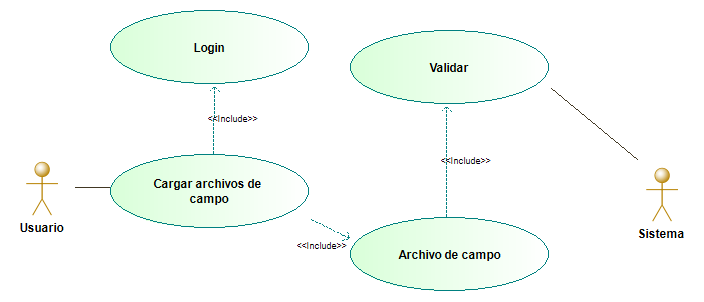
\includegraphics[width=0.7\textwidth]{CU-3}
	\caption{Diagrama de caso de uso CU-03.}
	\label{fig:CU-3}
\end{figure}
\begin{longtable}[H]{@{}ll@{}}
\toprule
\begin{minipage}[b]{0.23\columnwidth}\raggedright\strut
\textbf{CU-03}\strut
\end{minipage} & \begin{minipage}[b]{0.71\columnwidth}\raggedright\strut
\textbf{Carga de archivo de campo}\strut
\end{minipage}\tabularnewline
\midrule
\endhead
\begin{minipage}[t]{0.23\columnwidth}\raggedright\strut
\textbf{Versión}\strut
\end{minipage} & \begin{minipage}[t]{0.71\columnwidth}\raggedright\strut
1.0\strut
\end{minipage}\tabularnewline
\begin{minipage}[t]{0.23\columnwidth}\raggedright\strut
\textbf{Autor}\strut
\end{minipage} & \begin{minipage}[t]{0.71\columnwidth}\raggedright\strut
José Eduardo Risco Sánchez-Cortés\strut
\end{minipage}\tabularnewline
\begin{minipage}[t]{0.23\columnwidth}\raggedright\strut
\textbf{Requisitos asociados}\strut
\end{minipage} & \begin{minipage}[t]{0.71\columnwidth}\raggedright\strut
RF-3,RF-3.1, RF-2\strut
\end{minipage}\tabularnewline
\begin{minipage}[t]{0.23\columnwidth}\raggedright\strut
\textbf{Descripción}\strut
\end{minipage} & \begin{minipage}[t]{0.71\columnwidth}\raggedright\strut
Permite al usuario cargar un archivo de campo.\strut
\end{minipage}\tabularnewline
\begin{minipage}[t]{0.23\columnwidth}\raggedright\strut
\textbf{Precondición}\strut
\end{minipage} & \begin{minipage}[t]{0.71\columnwidth}\raggedright\strut
El usuario debe estar logeado.\\
El archivo debe tener extensión txt o csv.

\end{minipage}\tabularnewline
\begin{minipage}[t]{0.23\columnwidth}\raggedright\strut
\textbf{Acciones}\strut
\end{minipage} & \begin{minipage}[t]{0.71\columnwidth}%\raggedright\strut
\begin{enumerate}
\def\labelenumi{\arabic{enumi}.}
\tightlist
\item
  El usuario selecciona el archivo de campo, bien a través del botón \emph{Browse}, o arrastrando el archivo hasta la caja \emph{Topographical File data}.
\item
  El nombre del archivo aparece en la caja \emph{Topographical File data}.
\item
  El usuario confirma la carga con el botón \emph{Upload}
\end{enumerate}%\strut
\end{minipage}\tabularnewline
\begin{minipage}[t]{0.23\columnwidth}\raggedright\strut
\textbf{Postcondición}\strut
\end{minipage} & \begin{minipage}[t]{0.71\columnwidth}\raggedright\strut
La aplicación cambia a la pantalla de \emph{Upload File}
\end{minipage}\tabularnewline
\begin{minipage}[t]{0.23\columnwidth}%\raggedright\strut
\textbf{Excepciones}\strut
\end{minipage} & \begin{minipage}[t]{0.71\columnwidth}%\raggedright\strut
\begin{itemize}
\tightlist
\item
  mensaje: \textit{Topographic data file has the following errors...}
\item
  mensaje: \textit{Topographic data file is empty.}
\item
  mensaje: \textit{The number of points with \textit{TC} code in the topographic data file is not multiple of 2.}  
\item
  mensaje: \textit{The number of points with \textit{TR} code in the topographic data file is not multiple of 3.}  
\end{itemize}\strut
\end{minipage}\tabularnewline
\begin{minipage}[t]{0.23\columnwidth}%\raggedright\strut
\textbf{Importancia}\strut
\end{minipage} & \begin{minipage}[t]{0.71\columnwidth}%\raggedright\strut
Alta\strut
\end{minipage}\tabularnewline
\bottomrule
\caption{CU-03 Carga de archivo de campo.}
\end{longtable}


\imagen{CU-4}{Diagrama de caso de uso CU-04}

\begin{longtable}[H]{@{}ll@{}}
\toprule
\begin{minipage}[b]{0.23\columnwidth}\raggedright\strut
\textbf{CU-04}\strut
\end{minipage} & \begin{minipage}[b]{0.71\columnwidth}\raggedright\strut
\textbf{Carga de archivo de configuración}\strut
\end{minipage}\tabularnewline
\midrule
\endhead
\begin{minipage}[t]{0.23\columnwidth}\raggedright\strut
\textbf{Versión}\strut
\end{minipage} & \begin{minipage}[t]{0.71\columnwidth}\raggedright\strut
1.0\strut
\end{minipage}\tabularnewline
\begin{minipage}[t]{0.23\columnwidth}\raggedright\strut
\textbf{Autor}\strut
\end{minipage} & \begin{minipage}[t]{0.71\columnwidth}\raggedright\strut
José Eduardo Risco Sánchez-Cortés\strut
\end{minipage}\tabularnewline
\begin{minipage}[t]{0.23\columnwidth}\raggedright\strut
\textbf{Requisitos asociados}\strut
\end{minipage} & \begin{minipage}[t]{0.71\columnwidth}\raggedright\strut
RF-3,RF-3.1,RF-3.2, RF-2\strut
\end{minipage}\tabularnewline
\begin{minipage}[t]{0.23\columnwidth}\raggedright\strut
\textbf{Descripción}\strut
\end{minipage} & \begin{minipage}[t]{0.71\columnwidth}\raggedright\strut
Permite al usuario cargar un archivo de configuración de la conversión.\strut
\end{minipage}\tabularnewline
\begin{minipage}[t]{0.23\columnwidth}\raggedright\strut
\textbf{Precondición}\strut
\end{minipage} & \begin{minipage}[t]{0.71\columnwidth}\raggedright\strut
El usuario debe estar logeado.\\
El archivo debe tener extensión txt o csv.\\
El archivo de campo debe estar seleccionado

\end{minipage}\tabularnewline
\begin{minipage}[t]{0.23\columnwidth}\raggedright\strut
\textbf{Acciones}\strut
\end{minipage} & \begin{minipage}[t]{0.71\columnwidth}\raggedright\strut
\begin{enumerate}
\def\labelenumi{\arabic{enumi}.}
\tightlist
\item
  El usuario selecciona el archivo de configuración, bien a través del botón \emph{Browse}, o arrastrando el archivo hasta la caja \emph{User Configuration File}.
\item
  El nombre del archivo aparece en la caja \emph{User Configuration File}.
\item
  El usuario confirma la carga con el botón \emph{Upload}
   
\end{enumerate}\strut
\end{minipage}\tabularnewline
\begin{minipage}[t]{0.23\columnwidth}\raggedright\strut
\textbf{Postcondición}\strut
\end{minipage} & \begin{minipage}[t]{0.71\columnwidth}\raggedright\strut
\begin{enumerate}
\def\labelenumi{\arabic{enumi}.}
\tightlist
\item Postcondición 1, no se muestran errores:
La aplicación cambia a la pantalla de \emph{Upload File}\\
Aparece cargada la configuración en la tabla de la interfaz.\\
\item Postcondición 2, e muestran errores:
La aplicación cambia a la pantalla de \emph{Upload File}\\
Aparece cargada la configuración en la tabla de la interfaz.\\
Pueden mostrarse estos 2 errores:
\begin{itemize}
\tightlist
\item
  mensaje: \textit{User configuration has different colors on the same lines.}  
\item
  mensaje: \textit{Some color of the user configuration is not a CAD color.}      
\end{itemize}\strut  
Estos errores se deben subsanar por parte del usuario en esta pantalla sin necesidad de volver a cargar el archivo.
   
\end{enumerate}\strut


\end{minipage}\tabularnewline
\begin{minipage}[t]{0.23\columnwidth}\raggedright\strut
\textbf{Excepciones}\strut
\end{minipage} & \begin{minipage}[t]{0.71\columnwidth}\raggedright\strut
\begin{itemize}
\tightlist
\item
  mensaje: \textit{User configuration file file has the following errors...}
\item
  mensaje: \textit{User configuration file is empty.}
\item
  mensaje: \textit{User configuration file has duplicate items on different lines.}  

  
\end{itemize}\strut
\end{minipage}\tabularnewline
\begin{minipage}[t]{0.23\columnwidth}\raggedright\strut
\textbf{Importancia}\strut
\end{minipage} & \begin{minipage}[t]{0.71\columnwidth}\raggedright\strut
Alta\strut
\end{minipage}\tabularnewline
\bottomrule
\caption{CU-04 Carga de archivo de configuración.}
\end{longtable}

\begin{figure}[H]
	\centering
	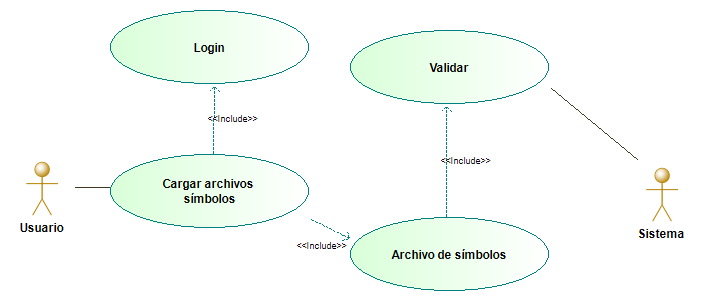
\includegraphics[width=0.7\textwidth]{CU-5}
	\caption{Diagrama de caso de uso CU-05.}
	\label{fig:CU-5}
\end{figure}

%\imagen{CU-5}{Diagrama de caso de uso CU-05}

\begin{longtable}[H]{@{}ll@{}}
\toprule
\begin{minipage}[b]{0.23\columnwidth}\raggedright\strut
\textbf{CU-05}\strut
\end{minipage} & \begin{minipage}[b]{0.71\columnwidth}\raggedright\strut
\textbf{Carga de archivo de símbolos}\strut
\end{minipage}\tabularnewline
\midrule
\endhead
\begin{minipage}[t]{0.23\columnwidth}\raggedright\strut
\textbf{Versión}\strut
\end{minipage} & \begin{minipage}[t]{0.71\columnwidth}\raggedright\strut
1.0\strut
\end{minipage}\tabularnewline
\begin{minipage}[t]{0.23\columnwidth}\raggedright\strut
\textbf{Autor}\strut
\end{minipage} & \begin{minipage}[t]{0.71\columnwidth}\raggedright\strut
José Eduardo Risco Sánchez-Cortés\strut
\end{minipage}\tabularnewline
\begin{minipage}[t]{0.23\columnwidth}\raggedright\strut
\textbf{Requisitos asociados}\strut
\end{minipage} & \begin{minipage}[t]{0.71\columnwidth}\raggedright\strut
RF-3, RF-3.1, RF-3.3, RF-2\strut
\end{minipage}\tabularnewline
\begin{minipage}[t]{0.23\columnwidth}\raggedright\strut
\textbf{Descripción}\strut
\end{minipage} & \begin{minipage}[t]{0.71\columnwidth}\raggedright\strut
Permite al usuario cargar un archivo DXF con símbolos.\strut
\end{minipage}\tabularnewline
\begin{minipage}[t]{0.23\columnwidth}\raggedright\strut
\textbf{Precondición}\strut
\end{minipage} & \begin{minipage}[t]{0.71\columnwidth}\raggedright\strut
El usuario debe estar logeado.\\
El archivo debe tener extensión dxf.\\
El archivo de campo debe estar seleccionado

\end{minipage}\tabularnewline
\begin{minipage}[t]{0.23\columnwidth}\raggedright\strut
\textbf{Acciones}\strut
\end{minipage} & \begin{minipage}[t]{0.71\columnwidth}\raggedright\strut
\begin{enumerate}
\def\labelenumi{\arabic{enumi}.}
\tightlist
\item
  El usuario selecciona el archivo de símbolos, bien a través del botón \emph{Browse}, o arrastrando el archivo hasta la caja \emph{CAD Symbols File}.
\item
  El nombre del archivo aparece en la caja \emph{CAD Symbols File}.
\item
  El usuario confirma la carga con el botón \emph{Upload}
\end{enumerate}\strut
\end{minipage}\tabularnewline
\begin{minipage}[t]{0.23\columnwidth}\raggedright
\textbf{Postcondición}\strut
\end{minipage} & \begin{minipage}[t]{0.71\columnwidth}\raggedright\strut
La aplicación cambia a la pantalla de \emph{Upload File}
\end{minipage}\tabularnewline
\begin{minipage}[t]{0.23\columnwidth}\raggedright\strut
\textbf{Excepciones}
\end{minipage} & \begin{minipage}[t]{0.71\columnwidth}%\raggedright\strut
\begin{itemize}
\tightlist
\item
  mensaje: \textit{CAD symbols file does not contain blocks.}

\end{itemize}\strut
\end{minipage}\tabularnewline
\begin{minipage}[t]{0.23\columnwidth}\raggedright\strut
\textbf{Importancia}\strut
\end{minipage} & \begin{minipage}[t]{0.71\columnwidth}\raggedright\strut
Alta\strut
\end{minipage}\tabularnewline
\bottomrule
\caption{CU-05 Carga de archivo de símbolos.}
\end{longtable}

\begin{figure}[H]
	\centering
	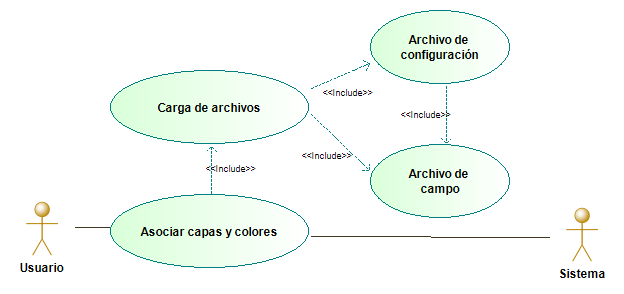
\includegraphics[width=0.7\textwidth]{CU-6}
	\caption{Diagrama de caso de uso CU-06.}
	\label{fig:CU-6}
\end{figure}


\begin{longtable}[H]{@{}ll@{}}
\toprule
\begin{minipage}[b]{0.23\columnwidth}\raggedright\strut
\textbf{CU-06}\strut
\end{minipage} & \begin{minipage}[b]{0.71\columnwidth}\raggedright\strut
\textbf{Asociar capas y colores}\strut
\end{minipage}\tabularnewline
\midrule
\endhead
\begin{minipage}[t]{0.23\columnwidth}\raggedright\strut
\textbf{Versión}\strut
\end{minipage} & \begin{minipage}[t]{0.71\columnwidth}\raggedright\strut
1.0\strut
\end{minipage}\tabularnewline
\begin{minipage}[t]{0.23\columnwidth}\raggedright\strut
\textbf{Autor}\strut
\end{minipage} & \begin{minipage}[t]{0.71\columnwidth}\raggedright\strut
José Eduardo Risco Sánchez-Cortés\strut
\end{minipage}\tabularnewline
\begin{minipage}[t]{0.23\columnwidth}\raggedright\strut
\textbf{Requisitos asociados}\strut
\end{minipage} & \begin{minipage}[t]{0.71\columnwidth}\raggedright\strut
RF-4, RF-4.1, RF-3, RF-3.1 \strut
\end{minipage}\tabularnewline
\begin{minipage}[t]{0.23\columnwidth}\raggedright\strut
\textbf{Descripción}\strut
\end{minipage} & \begin{minipage}[t]{0.71\columnwidth}\raggedright\strut
Permite al usuario asociar capas y colores, a los códigos extraídos del archivo de campo\strut
\end{minipage}\tabularnewline
\begin{minipage}[t]{0.23\columnwidth}\raggedright\strut
\textbf{Precondición}\strut
\end{minipage} & \begin{minipage}[t]{0.71\columnwidth}\raggedright\strut
El archivo de campo debe estar cargado.

\end{minipage}\tabularnewline
\begin{minipage}[t]{0.23\columnwidth}\raggedright\strut
\textbf{Acciones}\strut
\end{minipage} & \begin{minipage}[t]{0.71\columnwidth}\raggedright\strut
\begin{enumerate}
\def\labelenumi{\arabic{enumi}.}
\tightlist
\item
  El usuario introduce nombres de capas y selecciona colores, en la tabla, a través de la interfaz. En el caso de haber cargado un archivo de configuración esta aparecerá cargada en la tabla y se podrá modificar por el usuario.

\end{enumerate}\strut
\end{minipage}\tabularnewline
\begin{minipage}[t]{0.23\columnwidth}\raggedright\strut
\textbf{Postcondición}\strut
\end{minipage} & \begin{minipage}[t]{0.71\columnwidth}\raggedright\strut
  Los nombres de capas y colores seleccionados deben permanecer en la interfaz.
\end{minipage}\tabularnewline
\begin{minipage}[t]{0.23\columnwidth}\raggedright\strut
\textbf{Excepciones}\strut
\end{minipage} & \begin{minipage}[t]{0.71\columnwidth}\raggedright\strut
-\strut
\end{minipage}\tabularnewline
\begin{minipage}[t]{0.23\columnwidth}\raggedright\strut
\textbf{Importancia}\strut
\end{minipage} & \begin{minipage}[t]{0.71\columnwidth}\raggedright\strut
Alta\strut
\end{minipage}\tabularnewline
\bottomrule
\caption{CU-06 Asociar capas y colores.}
\end{longtable}
\strut
\imagen{CU-7}{Diagrama de caso de uso CU-07}
\strut
\begin{longtable}[H]{@{}ll@{}}
\toprule
\begin{minipage}[b]{0.23\columnwidth}\raggedright\strut
\textbf{CU-07}\strut
\end{minipage} & \begin{minipage}[b]{0.71\columnwidth}\raggedright\strut
\textbf{Asociar símbolos}\strut
\end{minipage}\tabularnewline
\midrule
\endhead
\begin{minipage}[t]{0.23\columnwidth}\raggedright\strut
\textbf{Versión}\strut
\end{minipage} & \begin{minipage}[t]{0.71\columnwidth}\raggedright\strut
1.0\strut
\end{minipage}\tabularnewline
\begin{minipage}[t]{0.23\columnwidth}\raggedright\strut
\textbf{Autor}\strut
\end{minipage} & \begin{minipage}[t]{0.71\columnwidth}\raggedright\strut
José Eduardo Risco Sánchez-Cortés\strut
\end{minipage}\tabularnewline
\begin{minipage}[t]{0.23\columnwidth}\raggedright\strut
\textbf{Requisitos asociados}\strut
\end{minipage} & \begin{minipage}[t]{0.71\columnwidth}\raggedright\strut
RF-4, RF-4.2, RF-3, RF-3.1\strut
\end{minipage}\tabularnewline
\begin{minipage}[t]{0.23\columnwidth}\raggedright\strut
\textbf{Descripción}\strut
\end{minipage} & \begin{minipage}[t]{0.71\columnwidth}\raggedright\strut
Permite al usuario asociar símbolos, a los códigos extraídos del archivo de campo\strut
\end{minipage}\tabularnewline
\begin{minipage}[t]{0.23\columnwidth}\raggedright\strut
\textbf{Precondición}\strut
\end{minipage} & \begin{minipage}[t]{0.71\columnwidth}\raggedright\strut
El archivo de campo debe estar cargado.\\
El archivo de símbolos debe estar cargado.

\end{minipage}\tabularnewline
\begin{minipage}[t]{0.23\columnwidth}\raggedright\strut
\textbf{Acciones}\strut
\end{minipage} & \begin{minipage}[t]{0.71\columnwidth}\raggedright\strut
\begin{enumerate}
\def\labelenumi{\arabic{enumi}.}
\tightlist
\item
 El usuario elige el símbolo a asociar a cada capa mediante un botón desplegable que contienen todos los símbolos disponibles.

\end{enumerate}\strut
\end{minipage}\tabularnewline
\begin{minipage}[t]{0.23\columnwidth}\raggedright\strut
\textbf{Postcondición}\strut
\end{minipage} & \begin{minipage}[t]{0.71\columnwidth}\raggedright\strut
  Los símbolos elegidos deben permanecer en la interfaz.
\end{minipage}\tabularnewline
\begin{minipage}[t]{0.23\columnwidth}\raggedright\strut
\textbf{Excepciones}\strut
\end{minipage} & \begin{minipage}[t]{0.71\columnwidth}\raggedright\strut
-\strut
\end{minipage}\tabularnewline
\begin{minipage}[t]{0.23\columnwidth}\raggedright\strut
\textbf{Importancia}\strut
\end{minipage} & \begin{minipage}[t]{0.71\columnwidth}\raggedright\strut
Alta\strut
\end{minipage}\tabularnewline
\bottomrule
\caption{CU-07 Asociar símbolos.}
\end{longtable}

\strut
\\
\\
\\


\imagen{CU-8}{Diagrama de caso de uso CU-08}

\strut

\begin{longtable}[H]{@{}ll@{}}
\toprule
\begin{minipage}[b]{0.23\columnwidth}\raggedright\strut
\textbf{CU-08}\strut
\end{minipage} & \begin{minipage}[b]{0.71\columnwidth}\raggedright\strut
\textbf{Elegir versión de CAD}\strut
\end{minipage}\tabularnewline
\midrule
\endhead
\begin{minipage}[t]{0.23\columnwidth}\raggedright\strut
\textbf{Versión}\strut
\end{minipage} & \begin{minipage}[t]{0.71\columnwidth}\raggedright\strut
1.0\strut
\end{minipage}\tabularnewline
\begin{minipage}[t]{0.23\columnwidth}\raggedright\strut
\textbf{Autor}\strut
\end{minipage} & \begin{minipage}[t]{0.71\columnwidth}\raggedright\strut
José Eduardo Risco Sánchez-Cortés\strut
\end{minipage}\tabularnewline
\begin{minipage}[t]{0.23\columnwidth}\raggedright\strut
\textbf{Requisitos asociados}\strut
\end{minipage} & \begin{minipage}[t]{0.71\columnwidth}\raggedright\strut
RF-4, RF-4.3, RF-3, RF-3.1\strut
\end{minipage}\tabularnewline
\begin{minipage}[t]{0.23\columnwidth}\raggedright\strut
\textbf{Descripción}\strut
\end{minipage} & \begin{minipage}[t]{0.71\columnwidth}\raggedright\strut
Permite al usuario elegir la versión de CAD para el archivo DXF generado\strut
\end{minipage}\tabularnewline
\begin{minipage}[t]{0.23\columnwidth}\raggedright\strut
\textbf{Precondición}\strut
\end{minipage} & \begin{minipage}[t]{0.71\columnwidth}\raggedright\strut
El archivo de campo debe estar cargado.\\
Deben ser accesibles las versiones de CAD disponibles. 
\end{minipage}\tabularnewline
\begin{minipage}[t]{0.23\columnwidth}\raggedright\strut
\textbf{Acciones}\strut
\end{minipage} & \begin{minipage}[t]{0.71\columnwidth}\raggedright\strut
\begin{enumerate}
\def\labelenumi{\arabic{enumi}.}
\tightlist
\item
 El usuario elige la versión de CAD mediante un botón desplegable que contienen todos los símbolos disponibles.
\end{enumerate}\strut
\end{minipage}\tabularnewline
\begin{minipage}[t]{0.23\columnwidth}\raggedright\strut
\textbf{Postcondición}\strut
\end{minipage} & \begin{minipage}[t]{0.71\columnwidth}\raggedright\strut
  La versión elegida debe permanecer en la interfaz.
\end{minipage}\tabularnewline
\begin{minipage}[t]{0.23\columnwidth}\raggedright\strut
\textbf{Excepciones}\strut
\end{minipage} & \begin{minipage}[t]{0.71\columnwidth}\raggedright\strut
-\strut
\end{minipage}\tabularnewline
\begin{minipage}[t]{0.23\columnwidth}\raggedright\strut
\textbf{Importancia}\strut
\end{minipage} & \begin{minipage}[t]{0.71\columnwidth}\raggedright\strut
Alta\strut
\end{minipage}\tabularnewline
\bottomrule
\caption{CU-08 Elegir versión de CAD.}
\end{longtable}
\strut

\imagen{CU-9}{Diagrama de caso de uso CU-09}

\strut
\begin{longtable}[H]{@{}ll@{}}
\toprule
\begin{minipage}[b]{0.23\columnwidth}\raggedright\strut
\textbf{CU-09}\strut
\end{minipage} & \begin{minipage}[b]{0.71\columnwidth}\raggedright\strut
\textbf{Dar nombre al archivo DXF generado}\strut
\end{minipage}\tabularnewline
\midrule
\endhead
\begin{minipage}[t]{0.23\columnwidth}\raggedright\strut
\textbf{Versión}\strut
\end{minipage} & \begin{minipage}[t]{0.71\columnwidth}\raggedright\strut
1.0\strut
\end{minipage}\tabularnewline
\begin{minipage}[t]{0.23\columnwidth}\raggedright\strut
\textbf{Autor}\strut
\end{minipage} & \begin{minipage}[t]{0.71\columnwidth}\raggedright\strut
José Eduardo Risco Sánchez-Cortés\strut
\end{minipage}\tabularnewline
\begin{minipage}[t]{0.23\columnwidth}\raggedright\strut
\textbf{Requisitos asociados}\strut
\end{minipage} & \begin{minipage}[t]{0.71\columnwidth}\raggedright\strut
RF-4, RF-4.4, RF-3, RF-3.1\strut
\end{minipage}\tabularnewline
\begin{minipage}[t]{0.23\columnwidth}\raggedright\strut
\textbf{Descripción}\strut
\end{minipage} & \begin{minipage}[t]{0.71\columnwidth}\raggedright\strut
Permite al usuario dar un nombre personalizado al archivo DXF generado\strut
\end{minipage}\tabularnewline
\begin{minipage}[t]{0.23\columnwidth}\raggedright\strut
\textbf{Precondición}\strut
\end{minipage} & \begin{minipage}[t]{0.71\columnwidth}\raggedright\strut
El archivo de campo debe estar cargado.\\
\end{minipage}\tabularnewline
\begin{minipage}[t]{0.23\columnwidth}\raggedright\strut
\textbf{Acciones}\strut
\end{minipage} & \begin{minipage}[t]{0.71\columnwidth}\raggedright\strut
\begin{enumerate}
\def\labelenumi{\arabic{enumi}.}
\tightlist
\item
 El usuario escribe un nombre en la caja llamada \emph{Filename }
\item
El nombre del archivo aparece en la caja.

\end{enumerate}\strut
\end{minipage}\tabularnewline
\begin{minipage}[t]{0.23\columnwidth}\raggedright\strut
\textbf{Postcondición}\strut
\end{minipage} & \begin{minipage}[t]{0.71\columnwidth}\raggedright\strut
El nombre del archivo debe permanecer en la interfaz.
\end{minipage}\tabularnewline
\begin{minipage}[t]{0.23\columnwidth}\raggedright\strut
\textbf{Excepciones}\strut
\end{minipage} & \begin{minipage}[t]{0.71\columnwidth}\raggedright\strut
-\strut
\end{minipage}\tabularnewline
\begin{minipage}[t]{0.23\columnwidth}\raggedright\strut
\textbf{Importancia}\strut
\end{minipage} & \begin{minipage}[t]{0.71\columnwidth}\raggedright\strut
Media\strut
\end{minipage}\tabularnewline
\bottomrule
\caption{CU-09 Dar nombre al archivo DXF generado.}
\end{longtable}
\strut
\\
\\
\\
\\
\begin{figure}[H]
	\centering
	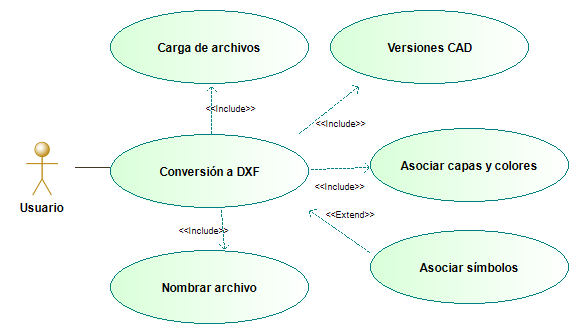
\includegraphics[width=0.7\textwidth]{CU-10}
	\caption{Diagrama de caso de uso CU-10.}
	\label{fig:CU-10}
\end{figure}
%\imagen{CU-10}{Diagrama de caso de uso CU-10}


\begin{longtable}[H]{@{}ll@{}}
\toprule
\begin{minipage}[b]{0.23\columnwidth}\raggedright\strut
\textbf{CU-10}\strut
\end{minipage} & \begin{minipage}[b]{0.71\columnwidth}\raggedright\strut
\textbf{Conversión a DXF}\strut
\end{minipage}\tabularnewline
\midrule
\endhead
\begin{minipage}[t]{0.23\columnwidth}\raggedright\strut
\textbf{Versión}\strut
\end{minipage} & \begin{minipage}[t]{0.71\columnwidth}\raggedright\strut
1.0\strut
\end{minipage}\tabularnewline
\begin{minipage}[t]{0.23\columnwidth}\raggedright\strut
\textbf{Autor}\strut
\end{minipage} & \begin{minipage}[t]{0.71\columnwidth}\raggedright\strut
José Eduardo Risco Sánchez-Cortés\strut
\end{minipage}\tabularnewline
\begin{minipage}[t]{0.23\columnwidth}\raggedright\strut
\textbf{Requisitos asociados}\strut
\end{minipage} & \begin{minipage}[t]{0.71\columnwidth}\raggedright\strut
RF-4, RF-4.1,RF-4.2,RF-4.3, RF-4.4, RF-3, RF-3.1\, RF-3.2, RF-3.3\strut
\end{minipage}\tabularnewline
\begin{minipage}[t]{0.23\columnwidth}\raggedright\strut
\textbf{Descripción}\strut
\end{minipage} & \begin{minipage}[t]{0.71\columnwidth}\raggedright\strut
Permite al usuario generar un archivo DXF \strut
\end{minipage}\tabularnewline
\begin{minipage}[t]{0.23\columnwidth}\raggedright\strut
\textbf{Precondición}\strut
\end{minipage} & \begin{minipage}[t]{0.71\columnwidth}\raggedright\strut
El archivo de campo debe estar cargado.\\
\end{minipage}\tabularnewline
\begin{minipage}[t]{0.23\columnwidth}\raggedright\strut
\textbf{Acciones}\strut
\end{minipage} & \begin{minipage}[t]{0.71\columnwidth}\raggedright\strut
\begin{enumerate}
\def\labelenumi{\arabic{enumi}.}
\tightlist
\item
  El usuario confirma la conversión con el botón \emph{Convert}
\end{enumerate}\strut
\end{minipage}\tabularnewline
\begin{minipage}[t]{0.23\columnwidth}\raggedright\strut
\textbf{Postcondición}\strut
\end{minipage} & \begin{minipage}[t]{0.71\columnwidth}\raggedright\strut
La aplicación cambia a la pantalla de \emph{Download File}\\
mensaje: \emph{File successfully converted!}
\end{minipage}\tabularnewline
\begin{minipage}[t]{0.23\columnwidth}\raggedright\strut
\textbf{Excepciones}\strut
\end{minipage} & \begin{minipage}[t]{0.71\columnwidth}\raggedright\strut
\begin{itemize}
\tightlist

\item
  mensaje: \textit{User configuration file has duplicate items on different lines.}  
\item
  mensaje: \textit{User configuration has different colors on the same lines.} 

\end{itemize}\strut
\end{minipage}\tabularnewline
\begin{minipage}[t]{0.23\columnwidth}\raggedright\strut
\textbf{Importancia}\strut
\end{minipage} & \begin{minipage}[t]{0.71\columnwidth}\raggedright\strut
Alta\strut
\end{minipage}\tabularnewline
\bottomrule
\caption{CU-10 Conversión a DXF.}
\end{longtable}


%\imagen{CU-11}{Diagrama de caso de uso CU-11}
\begin{figure}[H]
	\centering
	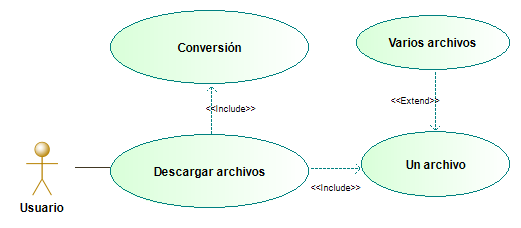
\includegraphics[width=0.7\textwidth]{CU-11}
	\caption{Diagrama de caso de uso CU-11.}
	\label{fig:CU-11}
\end{figure}

\begin{longtable}[H]{@{}ll@{}}
\toprule
\begin{minipage}[b]{0.23\columnwidth}\raggedright\strut
\textbf{CU-11}\strut
\end{minipage} & \begin{minipage}[b]{0.71\columnwidth}\raggedright\strut
\textbf{Descargar archivos}\strut
\end{minipage}\tabularnewline
\midrule
\endhead
\begin{minipage}[t]{0.23\columnwidth}\raggedright\strut
\textbf{Versión}\strut
\end{minipage} & \begin{minipage}[t]{0.71\columnwidth}\raggedright\strut
1.0\strut
\end{minipage}\tabularnewline
\begin{minipage}[t]{0.23\columnwidth}\raggedright\strut
\textbf{Autor}\strut
\end{minipage} & \begin{minipage}[t]{0.71\columnwidth}\raggedright\strut
José Eduardo Risco Sánchez-Cortés\strut
\end{minipage}\tabularnewline
\begin{minipage}[t]{0.23\columnwidth}\raggedright\strut
\textbf{Requisitos asociados}\strut
\end{minipage} & \begin{minipage}[t]{0.71\columnwidth}\raggedright\strut
RF-5, RF-4, RF-4.1,RF-4.2,RF-4.3, RF-4.4\strut
\end{minipage}\tabularnewline
\begin{minipage}[t]{0.23\columnwidth}\raggedright\strut
\textbf{Descripción}\strut
\end{minipage} & \begin{minipage}[t]{0.71\columnwidth}\raggedright\strut
Permite al usuario descargar a su equipo los archivos generados. \strut
\end{minipage}\tabularnewline
\begin{minipage}[t]{0.23\columnwidth}\raggedright\strut
\textbf{Precondición}\strut
\end{minipage} & \begin{minipage}[t]{0.71\columnwidth}\raggedright\strut
Deben existir archivos convertidos a DXF.\\
\end{minipage}\tabularnewline
\begin{minipage}[t]{0.23\columnwidth}\raggedright\strut
\textbf{Acciones}\strut
\end{minipage} & \begin{minipage}[t]{0.71\columnwidth}\raggedright
\begin{enumerate}
\def\labelenumi{\arabic{enumi}.}
\tightlist
\item
  El usuario puede elegir descargar un archivo individualmente.
\begin{itemize}
\tightlist
\item
  El usuario pulsa sobre el archivo a descargar. 
\item
  El archivo se descarga correctamente con formato dxf.
\end{itemize}
\item
  El usuario puede elegir descargar varios archivos a la vez.
\begin{itemize}
\tightlist
\item
  El usuario pulsa sobre el botón \emph{Download all}. 
\item
  El archivo se descarga correctamente con formato comprimido zip.
\end{itemize}
\end{enumerate}\strut
\end{minipage}\tabularnewline
\begin{minipage}[t]{0.23\columnwidth}\raggedright\strut
\textbf{Postcondición}\strut
\end{minipage} & \begin{minipage}[t]{0.71\columnwidth}\raggedright\strut
La aplicación permanece la pantalla de \emph{Download File}
\end{minipage}\tabularnewline
\begin{minipage}[t]{0.23\columnwidth}\raggedright\strut
\textbf{Excepciones}\strut
\end{minipage} & \begin{minipage}[t]{0.71\columnwidth}\raggedright\strut
-\strut
\end{minipage}\tabularnewline
\begin{minipage}[t]{0.23\columnwidth}\raggedright\strut
\textbf{Importancia}\strut
\end{minipage} & \begin{minipage}[t]{0.71\columnwidth}\raggedright\strut
Alta\strut
\end{minipage}\tabularnewline
\bottomrule
\caption{CU-11 Descargar archivos.}
\end{longtable}
\strut


\imagen{CU-12}{Diagrama de caso de uso CU-12}

\begin{longtable}[H]{@{}ll@{}}
\toprule
\begin{minipage}[b]{0.23\columnwidth}\raggedright\strut
\textbf{CU-12}\strut
\end{minipage} & \begin{minipage}[b]{0.71\columnwidth}\raggedright\strut
\textbf{\emph{Logout}}\strut
\end{minipage}\tabularnewline
\midrule
\endhead
\begin{minipage}[t]{0.23\columnwidth}\raggedright\strut
\textbf{Versión}\strut
\end{minipage} & \begin{minipage}[t]{0.71\columnwidth}\raggedright\strut
1.0\strut
\end{minipage}\tabularnewline
\begin{minipage}[t]{0.23\columnwidth}\raggedright\strut
\textbf{Autor}\strut
\end{minipage} & \begin{minipage}[t]{0.71\columnwidth}\raggedright\strut
José Eduardo Risco Sánchez-Cortés\strut
\end{minipage}\tabularnewline
\begin{minipage}[t]{0.23\columnwidth}\raggedright\strut
\textbf{Requisitos asociados}\strut
\end{minipage} & \begin{minipage}[t]{0.71\columnwidth}\raggedright\strut
RF-6, RF-2\strut
\end{minipage}\tabularnewline
\begin{minipage}[t]{0.23\columnwidth}\raggedright\strut
\textbf{Descripción}\strut
\end{minipage} & \begin{minipage}[t]{0.71\columnwidth}\raggedright\strut
Permite al usuario cerrar la sesión. \strut
\end{minipage}\tabularnewline
\begin{minipage}[t]{0.23\columnwidth}\raggedright\strut
\textbf{Precondición}\strut
\end{minipage} & \begin{minipage}[t]{0.71\columnwidth}\raggedright\strut
El usuario debe estar \emph{logeado}.\\
\end{minipage}\tabularnewline
\begin{minipage}[t]{0.23\columnwidth}\raggedright\strut
\textbf{Acciones}\strut
\end{minipage} & \begin{minipage}[t]{0.71\columnwidth}\raggedright
\begin{enumerate}
\def\labelenumi{\arabic{enumi}.}
\tightlist
\item
  El usuario pulsa el botón \emph{Sign out}.
\item
  La aplicación va a la pantalla de bienvenida.

\end{enumerate}\strut
\end{minipage}\tabularnewline
\begin{minipage}[t]{0.23\columnwidth}\raggedright\strut
\textbf{Postcondición}\strut
\end{minipage} & \begin{minipage}[t]{0.71\columnwidth}\raggedright\strut
La aplicación cierra la sesión.
\end{minipage}\tabularnewline
\begin{minipage}[t]{0.23\columnwidth}\raggedright\strut
\textbf{Excepciones}\strut
\end{minipage} & \begin{minipage}[t]{0.71\columnwidth}\raggedright\strut
-\strut
\end{minipage}\tabularnewline
\begin{minipage}[t]{0.23\columnwidth}\raggedright\strut
\textbf{Importancia}\strut
\end{minipage} & \begin{minipage}[t]{0.71\columnwidth}\raggedright\strut
Alta\strut
\end{minipage}\tabularnewline
\bottomrule
\caption{CU-12 \emph{Logout}.}
\end{longtable}
\strut

\imagen{CU-13}{Diagrama de caso de uso CU-13}

\begin{longtable}[H]{@{}ll@{}}
\toprule
\begin{minipage}[b]{0.23\columnwidth}\raggedright\strut
\textbf{CU-12}\strut
\end{minipage} & \begin{minipage}[b]{0.71\columnwidth}\raggedright\strut
\textbf{Limpiar archivos}\strut
\end{minipage}\tabularnewline
\midrule
\endhead
\begin{minipage}[t]{0.23\columnwidth}\raggedright\strut
\textbf{Versión}\strut
\end{minipage} & \begin{minipage}[t]{0.71\columnwidth}\raggedright\strut
1.0\strut
\end{minipage}\tabularnewline
\begin{minipage}[t]{0.23\columnwidth}\raggedright\strut
\textbf{Autor}\strut
\end{minipage} & \begin{minipage}[t]{0.71\columnwidth}\raggedright\strut
José Eduardo Risco Sánchez-Cortés\strut
\end{minipage}\tabularnewline
\begin{minipage}[t]{0.23\columnwidth}\raggedright\strut
\textbf{Requisitos asociados}\strut
\end{minipage} & \begin{minipage}[t]{0.71\columnwidth}\raggedright\strut
RF-7, RF-6, RF-2\strut
\end{minipage}\tabularnewline
\begin{minipage}[t]{0.23\columnwidth}\raggedright\strut
\textbf{Descripción}\strut
\end{minipage} & \begin{minipage}[t]{0.71\columnwidth}\raggedright\strut
Permite al sistema eliminar los archivos usados durante la sesión. \strut
\end{minipage}\tabularnewline
\begin{minipage}[t]{0.23\columnwidth}\raggedright\strut
\textbf{Precondición}\strut
\end{minipage} & \begin{minipage}[t]{0.71\columnwidth}\raggedright\strut
El usuario debe estar \emph{logeado}.\\
El usuario debe haber subido archivos o realizado conversiones.\\
\end{minipage}\tabularnewline
\begin{minipage}[t]{0.23\columnwidth}\raggedright\strut
\textbf{Acciones}\strut
\end{minipage} & \begin{minipage}[t]{0.71\columnwidth}\raggedright
\begin{enumerate}
\def\labelenumi{\arabic{enumi}.}
\tightlist
\item
  El usuario pulsa el botón \emph{Sign out}.
\item
  La aplicación va a la pantalla de bienvenida.

\end{enumerate}\strut
\end{minipage}\tabularnewline
\begin{minipage}[t]{0.23\columnwidth}\raggedright\strut
\textbf{Postcondición}\strut
\end{minipage} & \begin{minipage}[t]{0.71\columnwidth}\raggedright\strut
La aplicación elimina todos los archivos utilizados en la sesión.
\end{minipage}\tabularnewline
\begin{minipage}[t]{0.23\columnwidth}\raggedright\strut
\textbf{Excepciones}\strut
\end{minipage} & \begin{minipage}[t]{0.71\columnwidth}\raggedright\strut
-\strut
\end{minipage}\tabularnewline
\begin{minipage}[t]{0.23\columnwidth}\raggedright\strut
\textbf{Importancia}\strut
\end{minipage} & \begin{minipage}[t]{0.71\columnwidth}\raggedright\strut
Media\strut
\end{minipage}\tabularnewline
\bottomrule
\caption{CU-13 Limpiar archivos.}
\end{longtable}
\strut